\chapter{Other concerns}
\section{The concern of DDOS attacks}

DDOS is the important issue for building DNS server.
\\

There are 2 sorts of DNS queries, recursive and iterative. At the beginning, users send queries to recursive servers, when recursive DNS servers receive requests, if they do not have the matched IP addresses, then recursive DNS servers can help users to ask authoritative DNS servers for getting IP addresses, then return results to users, that is the recursive query. 
\\

As for the iterative query, when authoritative DNS servers receive the queries from recursive DNS servers, if they do not have the matched IP addresses, they will give recursive servers the IP addresses of other authoritative DNS servers for querying, then recursive servers will ask other authoritative DNS servers, this type of querying is the iterative query \cite{What_is_recursive_DNS}.
\\

However, the recursive queries may cause DDOS attacks. The content of packet could be faked, the IP address of a sender can be changed to be the IP address of the victim. In case thousands of computers send recursive queries to DNS servers, and all IPs of sources are changed to be the IP of a victim, then those DNS servers will send thousands of responses to that victim. After that, the traffic in the victim would be too high then cause some problems  \cite{Why_recursive_dns_not_recommended_video}. This type of DDOS attack is called DNS amplification attack \cite{DNS_amplification}.
\\

\begin{figure}[hbt!]  
    \centering
    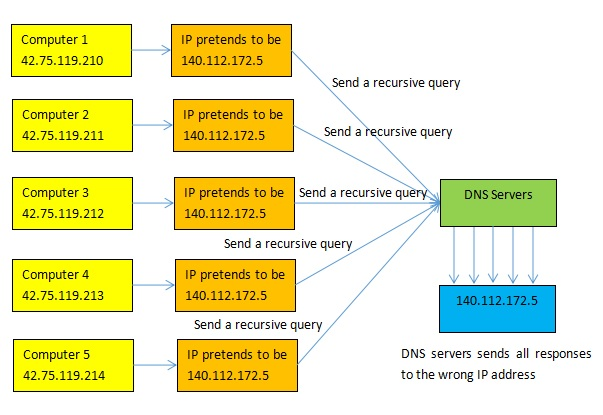
\includegraphics[width=0.8\textwidth]{figure/recursive-query-ddos.jpg}
    \caption{\em The DDOS attack in recursive DNS queries \cite{Why_recursive_dns_not_recommended_video} \label{fig:DDOS_attack}}
\end{figure}

Thus, restricting DNS queries may be the ideal method to prevent DNS amplification attacks, the implementation is to disable the recursion for everyone, only local queries are allowed to be processed \cite{Why_recursive_dns_not_recommended_web}.
\\

\begin{figure}[hbt!]  
    \centering
    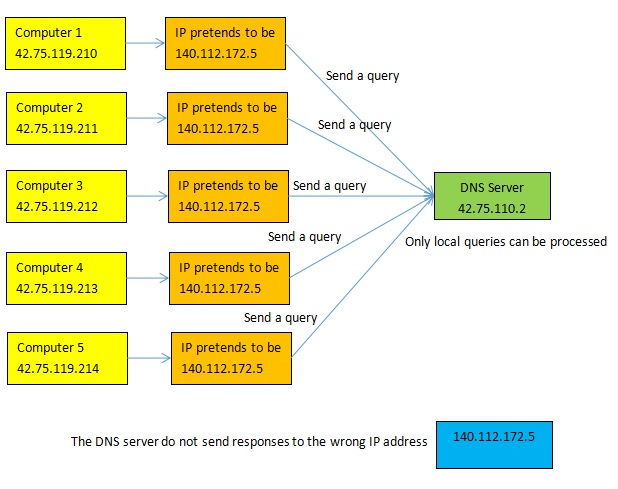
\includegraphics[width=0.8\textwidth]{figure/only_local_queries.jpg}
    \caption{\em Restricting DNS queries to prevent DNS amplification attacks \cite{Why_recursive_dns_not_recommended_video} \label{fig:restricting_DNS_queries}}
\end{figure}


\section{The required performance}

A DNS transaction contains many packets.

\section{The concern of disasters}

COVID-19
\\